\documentclass[border=3pt,tikz]{standalone}
\usepackage{physics}
\usepackage{bm}
\usepackage{tikz}
\usetikzlibrary{patterns,decorations.pathmorphing}
\usetikzlibrary{arrows.meta}
\usetikzlibrary{calc}
\tikzset{>=latex}

\colorlet{mydarkblue}{blue!50!black}
\colorlet{myblue}{blue!30}
\colorlet{mydarkred}{red!60!black}
\colorlet{myred}{red!30}
\colorlet{mydarkgreen}{green!60!black}
\colorlet{mygreen}{green!30}
\colorlet{mydarkorange}{yellow!40!red}
\colorlet{myorange}{yellow!80!red}
\colorlet{myyellow}{yellow!80}
\colorlet{mygrey}{black!15}
\colorlet{mydarkgrey}{black!50}

\tikzstyle{piston}=[blue!40!black,top color=blue!40!black!30,bottom color=blue!40!black!30,
                    middle color=blue!50!black!15,shading angle=0]
\tikzstyle{walldark}=[blue!25!black,top color=blue!20!black!12,bottom color=blue!20!black!20,shading angle=-30]
\tikzstyle{wall}=[blue!20!black,top color=blue!35!black!6,bottom color=blue!25!black!12,shading angle=30]

\tikzset{
  gasparticle/.pic={
    \tikzset{/gasparticle/.cd,#1}
    \draw[-{Latex[length=4,width=3]},green!60!black,thick] (0,0) -- (\vec);
    \node[circle,fill,inner sep=1.5,ball color=black!80!blue] at (0,0) {};
  }
  /gasparticle/.search also={/tikz},
  /gasparticle/.cd,
  vec/.store in=\vec, vec={90:0.5},
}

\begin{document}


% PISTON
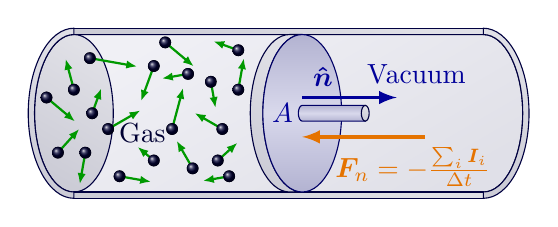
\begin{tikzpicture}
  \def\Ra{0.5}
  \def\Rb{1.0}
  \def\ra{0.05}
  \def\rb{0.1}
  \def\w{0.08} % wall thickness
  \def\x{2.9}  % piston position
  \def\L{5.2}  % container length
  \def\l{0.8}  % piston arm length
  \def\v{0.68} % velocity
  
  % WALL
  \draw[wall]
    (0,\Rb) -- (0,-\Rb) --++ (\L,0) arc (-90:90:{\Ra} and {\Rb}) -- cycle;
  \draw[walldark] (0,0) ellipse ({\Ra} and \Rb);
  
  % SHELL
  \draw[walldark]
    (0,\Rb) rectangle++ (\L,\w);
  \draw[walldark]
    (0,-\Rb) rectangle++ (\L,-\w);
  \draw[walldark]
    (\L,\Rb+\w) arc (90:-90:{\Ra+\w} and {\Rb+\w}) --++ (0,\w) arc (-90:90:{\Ra} and {\Rb}) -- cycle;
  \draw[walldark]
    (0,\Rb) arc (90:270:{\Ra} and {\Rb}) --++ (0,-\w) arc (-90:-270:{\Ra+\w} and {\Rb+\w}) -- cycle;
  
  % PISTON
  \draw[walldark]
    (\x,\Rb) arc (90:270:{\Ra} and {\Rb}) --++ (-2*\w,0) arc (-90:-270:{\Ra} and {\Rb}) -- cycle;
  \draw[piston] (\x,0) ellipse ({\Ra} and \Rb);
  \draw[piston]
    (\x,\rb) arc (90:270:{\ra} and {\rb}) --++ (\l,0) --++ (0,2*\rb) -- cycle;
  \draw[walldark] (\x+\l,0) ellipse ({\ra} and \rb);
  
  % LABELS
  \draw[<-,very thick,orange!90!black] (\x,-0.3*\Rb) --++ (0.3*\L,0)
    node[pos=0.9,below=0,orange!90!black] {$\bm{F}_n=-\frac{\sum_i\bm{I}_{i}}{\Delta t}$};
  \node[blue!60!black] at (\x-0.5*\Ra,0*\Rb) {$A$};      

  \draw[->, very thick,blue!60!black] (\x,0.2*\Rb)--++(1.5*\l,0) node[above,pos=0.22] {$\bm{\hat{n}}$};
  
  
  % GAS PARTICLE
  \pic at (-0.12*\x, 0.2*\Rb) {gasparticle={vec={ -40:0.7*\v}}};
  \pic at (-0.07*\x,-0.5*\Rb) {gasparticle={vec={  48:0.6*\v}}};
  \pic at ( 0.00*\x, 0.3*\Rb) {gasparticle={vec={ 105:0.6*\v}}};
  \pic at ( 0.05*\x,-0.5*\Rb) {gasparticle={vec={-100:0.6*\v}}};
  \pic at ( 0.08*\x, 0.0*\Rb) {gasparticle={vec={  70:0.5*\v}}};
  \pic at ( 0.07*\x, 0.7*\Rb) {gasparticle={vec={ -10:0.9*\v}}};
  \pic at ( 0.15*\x,-0.2*\Rb) {gasparticle={vec={  30:0.7*\v}}};
  \pic at ( 0.20*\x,-0.8*\Rb) {gasparticle={vec={ -10:0.6*\v}}};
  \pic at ( 0.35*\x, 0.6*\Rb) {gasparticle={vec={-110:0.7*\v}}};
  \pic at ( 0.35*\x,-0.6*\Rb) {gasparticle={vec={ 140:0.4*\v}}};
  \pic at ( 0.40*\x, 0.9*\Rb) {gasparticle={vec={ -40:0.7*\v}}};
  \pic at ( 0.43*\x,-0.2*\Rb) {gasparticle={vec={  75:0.8*\v}}};
  \pic at ( 0.50*\x, 0.5*\Rb) {gasparticle={vec={-170:0.5*\v}}};
  \pic at ( 0.52*\x,-0.7*\Rb) {gasparticle={vec={ 120:0.6*\v}}};
  \pic at ( 0.60*\x, 0.4*\Rb) {gasparticle={vec={ -80:0.5*\v}}};
  \pic at ( 0.63*\x,-0.6*\Rb) {gasparticle={vec={  42:0.5*\v}}};
  \pic at ( 0.65*\x,-0.2*\Rb) {gasparticle={vec={ 150:0.6*\v}}};
  \pic at ( 0.68*\x,-0.8*\Rb) {gasparticle={vec={ 190:0.5*\v}}};
  \pic at ( 0.72*\x, 0.8*\Rb) {gasparticle={vec={ 160:0.5*\v}}};
  \pic at ( 0.72*\x, 0.3*\Rb) {gasparticle={vec={  80:0.6*\v}}};

  % COMPARTMENT LABELS
  \node[black!80!blue] at (0.3*\x,-0.25*\Rb) {Gas};
  \node[blue!60!black] at (1.5*\x,0.5*\Rb) {Vacuum};
  
\end{tikzpicture}


% PISTON
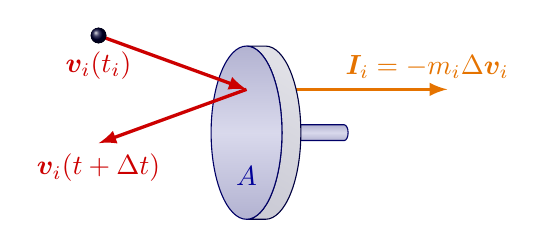
\begin{tikzpicture}
  \def\Ra{0.45}
  \def\Rb{1.10}
  \def\ra{0.05}
  \def\rb{0.1}
  \def\w{0.12}  % wall thickness
  \def\l{1}     % piston length
  \def\ang{160} % momentum angle
  \def\p{2}   % momentum length
  
  % PISTON
  %\draw[->, very thick,blue!60!black] (0,0)--++(0.9*\p,0) node[below,pos=1] {$\bm{\hat{n}}$};

  \draw[->,very thick,orange!90!black] (0*\w,{0.5*\Rb)}) --++ (2.55*\l,0)
    node[pos=0.9,above,orange!90!black] {$\bm{I}_{i}=-m_i\Delta \bm{v}_{i}$};
  \draw[piston]
    (2*\w,\rb) --++ (\l,0) arc (90:-90:{\ra} and {\rb}) --++ (-\l,0) -- cycle;
  
  %\draw[very thick,blue!60!black,dashed,opacity=0.5] (0,0)--++(0.8*\p,0);

  \draw[walldark]
    (0,\Rb) arc (90:-90:{\Ra} and {\Rb}) --++ (2*\w,0) arc (-90:90:{\Ra} and {\Rb}) -- cycle;
  \draw[piston] (0,0) ellipse ({\Ra} and \Rb);
  
  % GAS PARTICLE
  \draw[->,very thick,red!80!black]
  ($(0,0.5*\Rb)+(\ang:\p)$) node[below=2] {$\bm{v}_i(t_i)$} coordinate (I) -- (0,0.5*\Rb);
  \draw[->,very thick,red!80!black]
    (0,0.5*\Rb) -- ($(0,0.5*\Rb)+(-\ang:\p)$) node[below] {$\bm{v}_i(t+\Delta t)$};
  \node[circle,fill,inner sep=2,ball color=black!80!blue] at (I) {};

  % LABEL
  \node[blue!60!black] at (0,-0.5*\Rb) {$A$};
  %\draw[very thick,blue!60!black,dashed,opacity=0.5] (0,0)--++(0.22*\p,0);

\end{tikzpicture}


\end{document}
